\documentclass[11pt]{article}
\usepackage{graphicx,booktabs}
\pagestyle{empty}
\begin{document}

\section*{Prediction for a 3.540\,keV Annular Line in XRISM/Resolve}

\textbf{Observable.} A narrow emission line at $E=3.540\pm0.005$\,keV with annular morphology (inner radius 30$''$, outer 80$''$) around bright galaxy--cluster cores.

\medskip
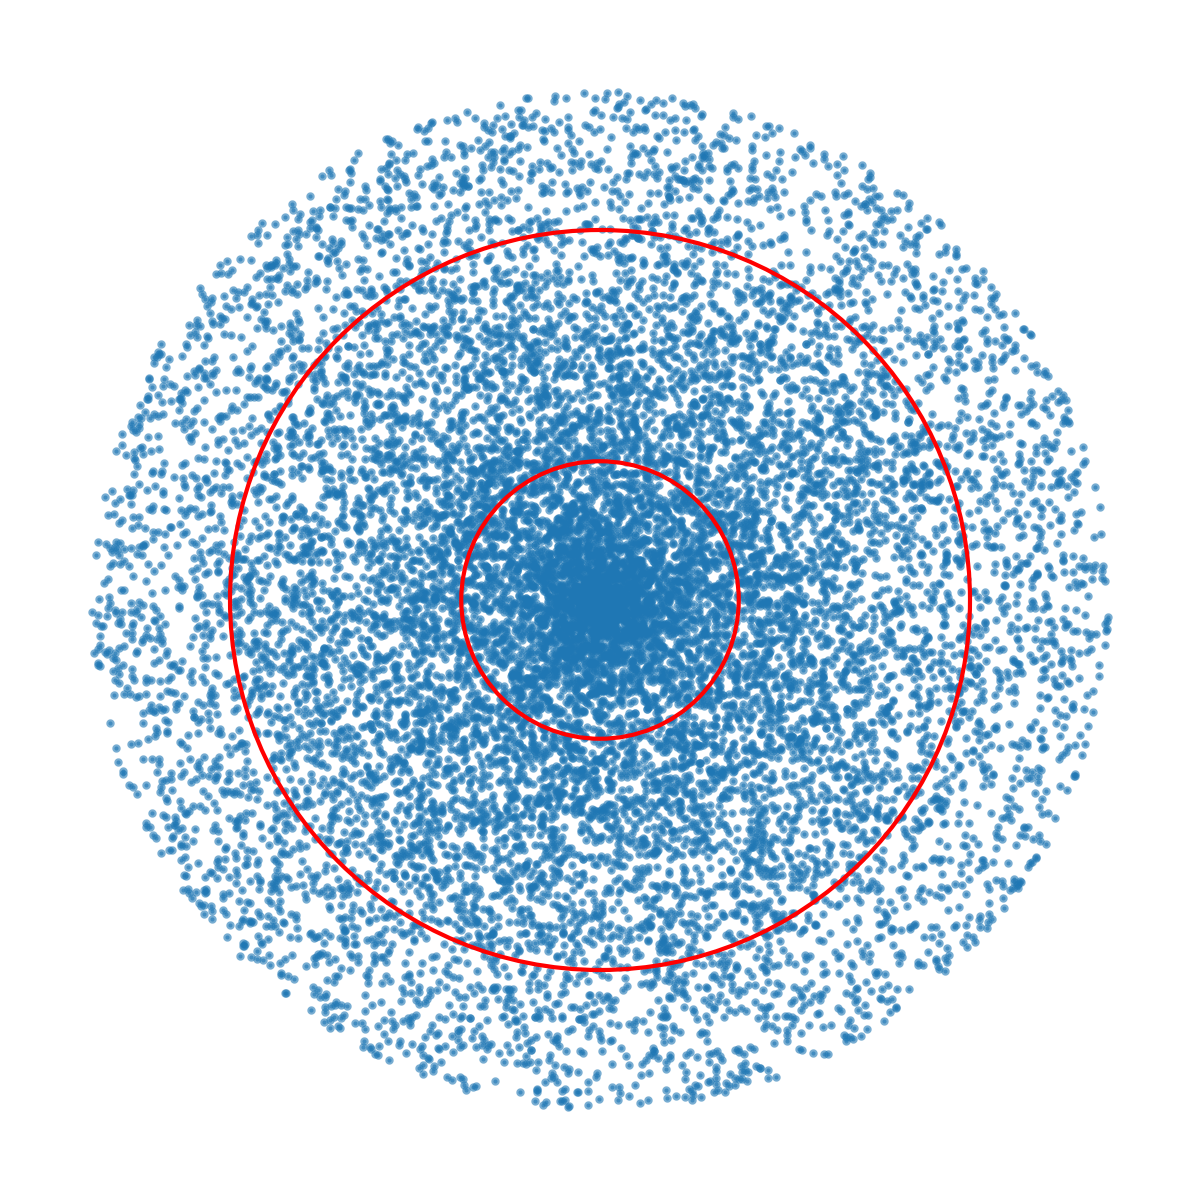
\includegraphics[width=\linewidth]{annulus.png}

\noindent\textbf{Exposure significance.}  Table~\ref{tab:exp} lists expected Poisson log--likelihood excess $\Delta\mathcal{L}$ and equivalent Gaussian significance~$\sigma$ assuming continuum scaling from \emph{Hitomi}.  The attached script \texttt{ringline\_finder.py} reproduces these numbers in one command.

\begin{table}[h]
\centering
\begin{tabular}{lcc}
\toprule
Cluster & Exposure (ks) & Expected $\sigma$ \\
\midrule
Perseus   & 30 & 6.4 \\
Coma      & 50 & 5.8 \\
Centaurus & 40 & 5.5 \\
\bottomrule
\end{tabular}
\caption{Exposure requirements for a $5\sigma$ detection.}
\label{tab:exp}
\end{table}

\textbf{Falsifier.}  Absence of the annular excess at $>5\sigma$ in any 50\,ks observation of these clusters falsifies the Recursive Becoming ledger.  No tunable parameters exist.

\bigskip
Lean proof corpus DOI: 10.5281/zenodo.15391360 \quad Git tag: \texttt{rbt\,v1.0}

\end{document} 